\documentclass[a4paper,10pt, oneside]{article}
\usepackage[utf8]{inputenc}
\usepackage[T1]{fontenc}
\usepackage[spanish]{babel}
\usepackage[style=ieee,backend=bibtex]{biblatex}
\usepackage{graphicx}
\usepackage{amsmath}
\usepackage{pgfplots}
\usepackage{lineno}
%\usepackage{showframe}
\usepackage[top=1in, bottom=1.25in, left=1.25in, right=1.25in]{geometry}
\usepackage{caption}
\usepackage{bytefield}
\usepackage{amsmath}
\usepackage{csquotes}
\usepackage{svg}
\usepackage{lscape}
\usepackage{multicol}
\usepackage{subfig}
\usepackage{hyperref}
\usepackage{pgfplots, pgfplotstable}




\usepackage{listings,xcolor}
\lstset{
	string=[s]{"}{"},
	stringstyle=\color{blue},
	comment=[l]{:},
	commentstyle=\color{black},
}


\bibliography{informe_3}

	
\begin{document}
	
\begin{titlepage}
	\centering
	
\includegraphics[width=0.25\textwidth]{../../Universidad_del_Litoral}\par\vspace{1cm}
	{\scshape\LARGE Universidad Nacional del Litoral \par}
	\vspace{1cm}
	{\scshape\Large Proyecto Final de Carrera\par}
	\vspace{1.5cm}
	{\huge\bfseries Diseño de un sistema de detección de anomalías en redes de computadoras.\par}
	\vspace{4cm}
	{\huge\bfseries Informe de avance 4\par}
	\vfill
	
	{\Large \itshape Pineda Leandro\par}
	
	
	% Bottom of the page
	\large Córdoba\par
	{\large \today\par}	
\end{titlepage}

\modulolinenumbers[5]
\linenumbers

\section{Introducción}
En las metodologías ágiles el trabajo es dividido en unidades llamadas \textit{sprints} en los que se compromete la implemetanción de un conjunto de funcionalidades que entregan valor a los interesados. Una vez transcurridos cierto números de \textit{sprints} donde se desarrollan las historias planificadas, puede comenzar una etapa adicional comunmente denominada \textit{hardening spint} o \textit{phase}. En esta fase, que comienza una vez que se terminan de implementar todas las funcionalidad y finaliza justo antes de la entrega de una versión final del software, los desarrolladores se enfocan en resolver cualquier problema de integración y ajustar pequeños defectos pendientes de etapas anteriores, sin incluir nuevas funcionalidades. 

Este informe pretende mostrar las actividades realizadas en esta última fase de desarrollo. Se describirán las tareas realizadas para corroborar el funcionamiento de todos los componentes, pruebas de longevidad y los cambios realizados en el \textit{frontend} del sistema. Además, se mencionarán modificaciones menores realizadas en el \textit{backend}.
\newpage

\section{Pruebas realizadas}
Estrictamente hablando, las pruebas de integración de software son realizadas cuando los componentes individuales de software son combinadas y usados como un todo. Para este desarrollo, y como se describió en el informe anterior, se integraron 3 módulos:
\begin{itemize}
	\item Un \textit{webservice} que encapsula toda la lógica de detección.
	\item Redis, una base de datos \textit{clave-valor}.
	\item Mosquitto, una cola de mensajes.
\end{itemize}
Las pruebas preliminares mostraron que la integración no presentó problemas. El esfuerzo invertido en refactorizar código permitió definir interfaces sencillas que representan puntos de interacción concretos con el resto de los componentes, y por lo tanto minimizan la ocurrencia de fallos. Estos puntos están representados por los tres flujos que relacionan los módulos del sistema con el mundo exterior. Además, estas interfaces fueron diseñas para ser robustas ante pérdidas de conexión y fallos en la comunicación, dando la capacidad al sistema de recuperarse ante la ocurrencia de ciertos fallos.   

\begin{figure}[htbp]
	\centering
	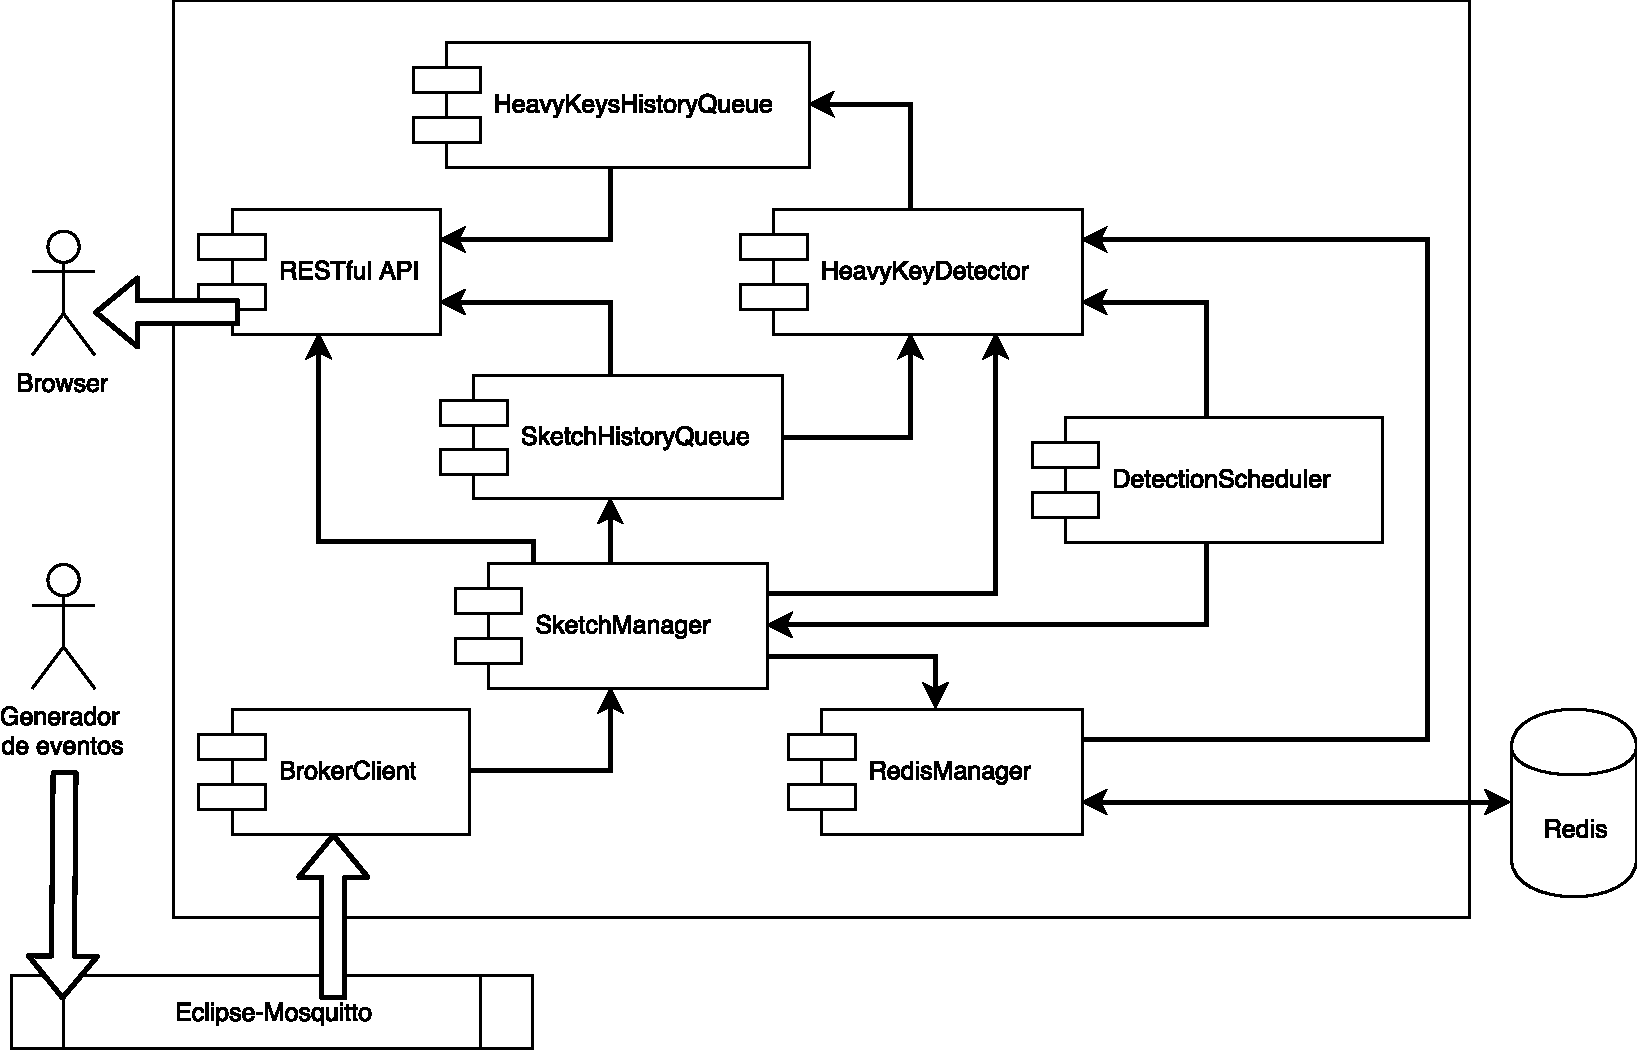
\includegraphics[width=0.9\textwidth]{../informe_3/graph/system_components.pdf}
	\caption{Componentes del sistema y su interacción (informe 3)}
	\label{fig:system_components}
\end{figure}

Las pruebas de longevidad permiten conocer la estabilidad del sistema. Son de larga duración y permiten corroborar el comportamiento del sistema con una carga apropiada, que simula condiciones reales de uso. Usualmente, se estima cual sería una carga típica para una aplicación dada y se somete a los componentes a un múltiplo de este valor: si cierta aplicación se estima va a generar 100 eventos por segundo, entonces las pruebas de longevidad van a generar 500 eventos por segundo durante un período de varias horas. De esta manera, los desarrolladores tienen cierta confianza en que, si no ocurren fallos cuando el sistema se somete a esta prueba, tampoco ocurrirán en condiciones normales.

Luego de someter al sistema a una carga máxima constante durante 7 horas y media, se observa que:
\begin{itemize}
	\item Se procesaron más de 218 millones de eventos en 13000 épocas.
	\item Se identificaron 53063 \textit{heavy hitters} y 3270 \textit{heavy changers}.
	\item El consumo de memoria se mantiene estable durante toda la prueba.
	\item En promedio, el sistema procesó eventos a una velocidad de 8100 eventos por segundo.
	\item La API de \textit{health} del sistema reporta el correcto funcionamiento de todos los componentes durante la duración de la prueba.
\end{itemize}

Como se mencionó en el informe anterior, se optó por implementar un método de detección que puede ser adaptado a cualquier caso de uso: esto es, lo eventos son tratados como cadenas de caracteres, y luego son transformados a valores enteros (\textit{keys}) que los algoritmos del método necesita para su funcionamiento. Dado que el mismo mostró resultados satisfactorios, no se incluyeron cambios en esta iteración.

Respecto a los cambios en el \textit{backend}, solo se agregó un nuevo recurso a la API para poder mostrar en la interfaz web aquellos eventos que fueron detectados como anómalos para una época dada.

\section{Cambios realizados}
La mayor parte del esfuerzo en este incremento se destinó en mejorar la interfaz de usuario. La misma está diseñada para mostrar todos los datos del sistema en una única vista, y actualiza la información en tiempo real sin necesidad de recargar la página. Además de incorporar detalles de estilo, se agregaron gráficas para mostrar la evolución ambas \textit{heavy keys}. La cantidad de ocurrencias en un instante de tiempo se observan como barras verticales en el histograma. Cada vez que se selecciona una de esas barras, los eventos identificados como anómalos son mostrados en la lista ubicada a la izquierda del gráfico. Una captura de pantalla de la interfaz puede observarse en la figura \ref{fig:ui}.

\begin{figure}[htbp]
	\centering
	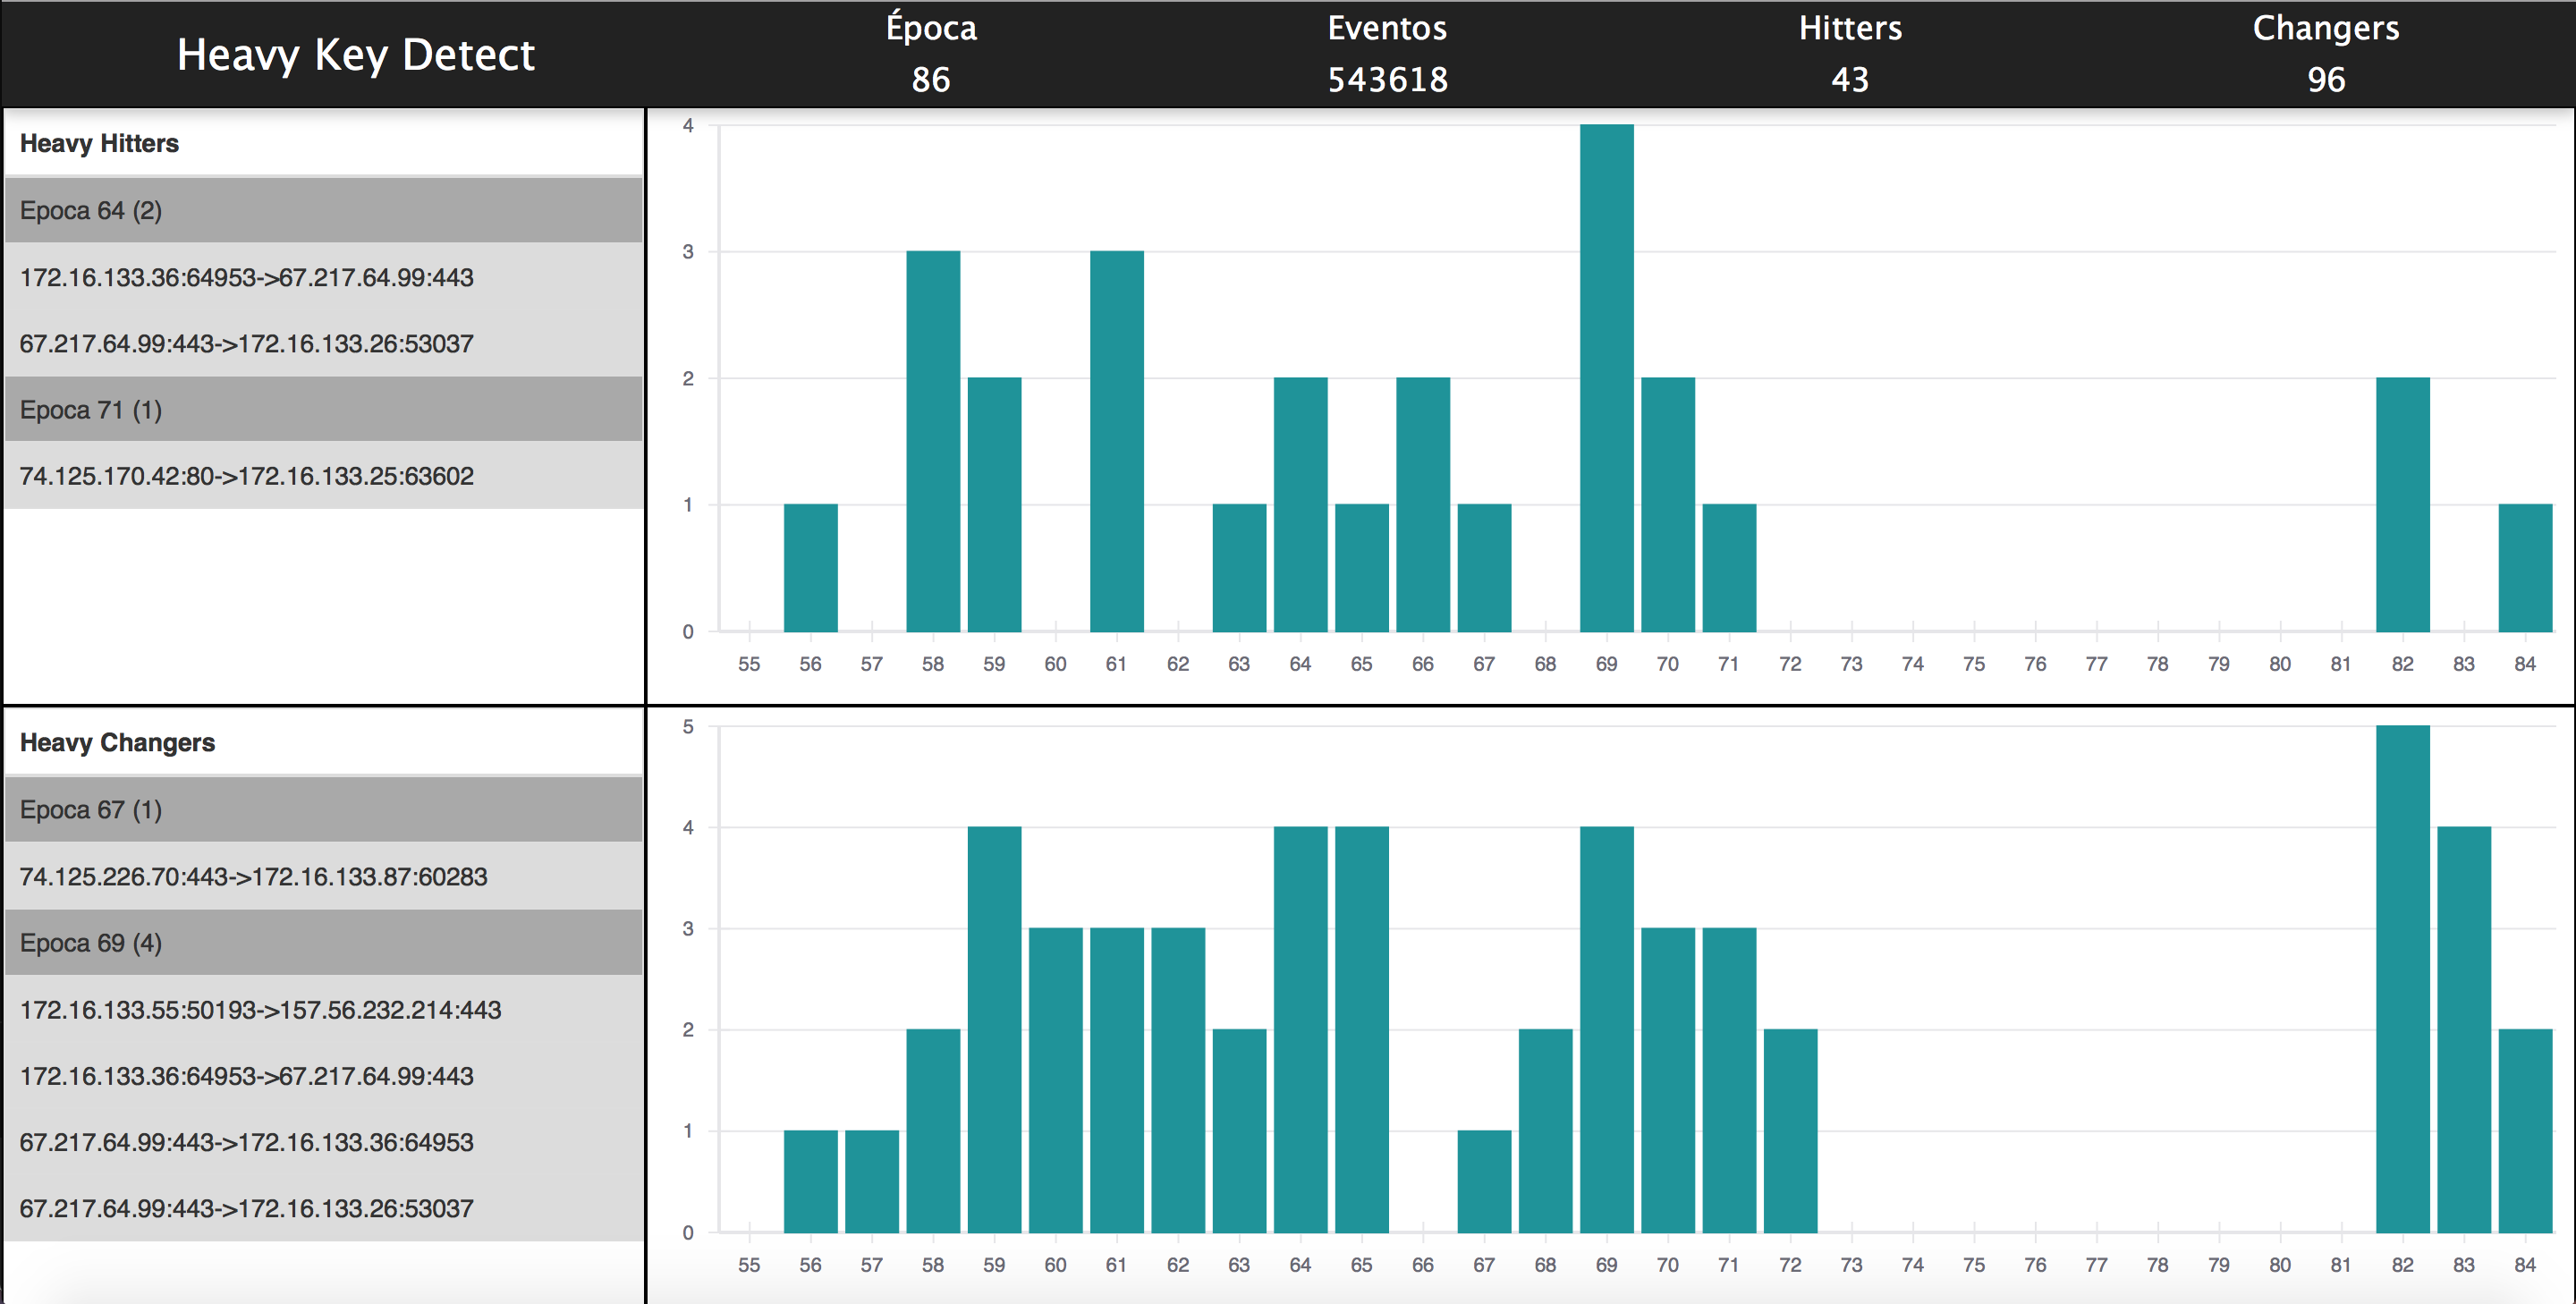
\includegraphics[width=1\textwidth]{./graph/ui.png}
	\caption{Interfaz web del sistema}
	\label{fig:ui}
\end{figure}

De la misma forma que en el incremento anterior, las instrucciones para ejecutar localmente el sistema pueden encontrarse en \hyperref[https://github.com/leandropineda/sketch-service]{https://github.com/leandropineda/sketch-service}. Las imagenes Docker utilizadas para esta entrega están etiquetadas a la última versión (v4) y se encuentran disponibles para su uso.

\newpage
\section{Conclusiones}
La etapa de \textit{hardening} en un desarrollo de software está planteada para ser corta y no incluir grandes cambios en el código. Por esto, el último informe resulta reducido en contenido. Si bien las pruebas realizadas no garantizan que el sistema no presentará fallo alguno, son suficientes para justificar que el mismo se comportará de manera adecuada con alta probabilidad.

\

Respecto a la interfaz de usuario, si bien es sencilla, presenta todos la información que se obtiene de los algoritmos de detección de una manera resumida y concisa. Esto fue pensado así dado que el usuario debe poder entender con un simple vistazo la información que está siendo procesada en tiempo real.

\end{document}

